%%%%%%%%%%%%%%%%%%%%%%%%%%%%%%%%% STUDY ON USAGE PATTERNS OF LLM USERS %%%%%%%%%%%%%%%%%%%%%%%%%%%%%%%%%
\section{Study on Usage Patterns of LLM Users}
\label{sec:study-on-usage-patterns-of-llm-users}

%%%%%%%%%%%%%%%%%%%%%%%%%%%%%%%%% RESEARCH OBJECTIVE %%%%%%%%%%%%%%%%%%%%%%%%%%%%%%%%%
\subsection{Research Objective}
\label{subsec:research-objective}
% Intro and Research Objective of the study goal, the methodology, and the individual
% steps that will be taken
The main outlined goal of our research is to gain a fundamental understanding of user behavior in conversation with Large Language Models.
This analysis includes identifying common patterns and strategies in those interactions.
Previous research indicates that users regularly face challenges and difficulties, especially
when trying to formulate effective prompts.
Through accumulation and analysis of qualified data samples we aim to identify and understand these
challenges,
as well as investigate the impact and effect of user behavior on the effectiveness of LLM responses.
Given the various kinds of available generative models, we want to examine differences in
prompting behavior according to model type as well.

Since related insights suggest that reformulating search queries is a popular strategy to improve
results, we want to investigate if users apply this strategy in LLM conversations as well. % TODO
% check if we really did this
Furthermore, we want to assess the extent to which users show awareness of effective prompt
formulation strategies, such as few-shot learning, and whether they rely on appropriate language
that is machine and not human directed, thus showing comprehension of the fundamental difference
between talking to a machine versus a human.

%%%%%%%%%%%%%%%%%%%%%%%%%%%%%%%%% RESEARCH METHOD %%%%%%%%%%%%%%%%%%%%%%%%%%%%%%%%%
\subsection{Research Method: ShareGPT and Midjourney}
\label{subsec:research-method:-sharegpt-and-midjourney}
% Information on the ShareGPT & Midjourney platforms, their user base, suitability for the
% study, and which data we are going to use
In order to obtain credible insights, we complement existing findings with real-world data.
Our study analyzes data samples from two different types of
LLMs.
First, we examine user interactions with ChatGPT, a generative NLP model, which has already been
described in more detail in Section~\ref{subsec:large-language-models-(llms)}.
These ChatGPT conversations were obtained from the website ShareGPT\cite{sharegpt_sharegpt_2023}.
ShareGPT is an open platform, that allows its community to publicly share interactions they have
had with the ChatGPT model.
As of today, ShareGPT has accumulated nearly 300.000 saved user conversations.
What makes ShareGPT particularly suitable for our use-case is the fact that the entire shared conversation
can be viewed by the observer as if they had personally conducted the interaction, allowing us to
gain a deeper understanding of the conversation dynamics and outcome.
\newline

Midjourney in contrast, is a platform that focuses on AI-based image generation.
Users can interact with the model through Discord\cite{} and submit individual requests. % TODO cite
In order to generate an illustration, users have to enter a descriptive prompt, similar to
ChatGPT\@.
The description typically includes everything that should appear in the picture, but may also
encompass the desired mood, drawing style, or composition of the image being generated.
Notably, the Midjourney Bot does not understand grammar, sentence structure, or specific words like
humans~\cite{}. % TODO cite
Midjourney's developers actively encourage using fewer, but more precise and impactful words when
prompting the model.
For example, they suggest using \("\)gigantic\("\) instead of \("\)big\("\) in order to achieve
better results. %TODO cite
This recommendation stems from the fact that fewer words in a prompt intensify the influence each
individual word has on the final outcome.
However, it is important to mention that users have to strike a balance.
An adequate amount of precise words is mandatory, because anything that is not specified may be
randomized.
In addition to purely textual prompts, the platform allows image inputs as well.
Users may provide an image as a guideline or basis including instructions about things to modify,
add, remove, or remodel.
The Midjourney platform on Discord has experienced rapid growth, and counts more than 17 million
members as of today.
\newline

In order to verify observations and findings we have presented in Section~\ref{sec:background-and-related-work},
we examine exemplary real-world user interaction samples in the following.
By randomly choosing 50 conversations from each ShareGPT's website as well as Midjourney's Discord
channel, we obtain a representative sample of average user behavior in both text and image targeting prompts.
We have defined dedicated categories according to which each sample is classified for both
the ChatGPT and Midjourney conversations.
For the language-focused ChatGPT conversations, the categories and specific sub-categories can be
seen in Table~\ref{tab:sharegpt-prompt-analysis-categories}.
Similarly, the categories and sub-categories for image-focused Midjourney prompts are listed
in Table~\ref{tab:midjourney-prompt-analysis-categories}.

For ShareGPT, we first of all classified the prompt by type, as in theory any kind of prompt is
possible, because users are solely constrained to natural language in any shape or form.
In the next category, it was of major interest what the user intended to achieve with their
individual prompts,
i.e.\ what they use the model for.
The categories prompt length and setting refer to the number of sentences in the user inputs, and
whether any examples were provided as part of the query.
Engagement refers to the amount of exchange in the interaction.
If the user prompted the model multiple times(at least twice) during the course of the
conversation, we considered the interaction multi turn, otherwise single turn.
The prompt's complexity gave us an idea whether users leverage ChatGPT for simple
tasks, that they may otherwise quickly research using a search engine, or if they pose complex
questions that require expert-level knowledge.
The refinement degree of the prompt revealed if users were generally content with the initial
answer of the LLM, or if further elaboration was needed.
Finally, we differentiated use of formal and informal language.
In general, when a single conversation consisted of multiple prompts, we labeled it based on the
most frequently observed category or significant behavior.

We classified Midjourney interactions using a similar approach.
First of all, we differentiated between image- and purely language-based inputs.
We then considered the length of the prompt, and whether it consisted solely of keywords, one
or more sentences, or a mix of both.
Next, we recorded the complexity of the whole prompt.
The Midjourney bot always generates four versions of the desired image.
It then allows users to either recreate variations or more detailed versions of one or more of
those four results.
Users can also re-execute the whole generation process.
We thus classified the prompt accordingly in the refinement category.
Finally, we recorded the clarity of the prompt and satisfaction levels based
on the observed user behavior.
If a user created variations or more detailed versions of the result, we assumed they were
generally satisfied.
Analogously, we assumed dissatisfaction if they regenerated the whole image.

% set linewidth 0,2281875 for \begin{tabular}{p{0.1\linewidth}p{0.81275\linewidth}}
\begin{table}[]
    \centering
    \caption{ShareGPT Prompt Analysis Categories}
    \begin{tabular}{@{}llll@{}}
        \toprule
        Type        & Intent        & Length             & Setting   \\ \midrule
        Question    & Information   & Long (5 + Sent.)   & Zero Shot \\
        Statement   & Advice        & Med (2 - 4 Sent.)  & One Shot  \\
        Command     & Clarification & Short (<= 1 Sent.) & Few Shot  \\
        Task-based  & Opinion       &                    &           \\
        & Suggestion    &                    &           \\
        & Entertainment &                    &           \\
        &               &                    &           \\
        \toprule
        Engagement  & Complexity    & Refinement         & Language  \\ \midrule
        Single Turn & Simple        & None               & Formal    \\
        Multi Turn  & Intermediate  & Once               & Informal  \\
        &               & Complex            &           \\ \bottomrule
    \end{tabular}
    \label{tab:sharegpt-prompt-analysis-categories}
\end{table}

\begin{table}[]
    \centering
    \caption{Midjourney Prompt Analysis Categories}
    \begin{tabular}{@{}llll@{}}
        \toprule
        Type         & Length            & Composition  & Complexity   \\ \midrule
        Language     & Long (12+ Words)  & Keyword-Only & Simple       \\
        Image        & Med (4-12 Words)  & Sentence     & Intermediate \\
        & Short (1-3 Words) & Mix          & Complex      \\
        \\
        \toprule
        Refinement          & Language & Clarity & Satisfaction \\
        \midrule
        None & Formal & Clear & Satisfied \\
        Variation          & Informal & Ambiguous & Dissatisfied \\
        Regeneration & & & Unclear \\
        \bottomrule
    \end{tabular}
    \label{tab:midjourney-prompt-analysis-categories}
\end{table}

%%%%%%%%%%%%%%%%%%%%%%%%%%%%%%%%% STUDY RESULTS %%%%%%%%%%%%%%%%%%%%%%%%%%%%%%%%%
\section{Study Results}
\label{sec:study-results}

%%%%%%%%%%%%%%%%%%%%%%%%%%%%%%%%% FINDINGS AND OBSERVABLE TRENDS %%%%%%%%%%%%%%%%%%%%%%%%%%%%%%%%%
\subsection{Findings and Observable Trends}
\label{subsec:findings-and-observable-trends}
% Listing of the results of the study, potentially segregated into categories that can be defined
% in advance
In the following section, we are going to break down the sample analysis results by category.
The distribution of the sub-categories in the individual categories Prompt Type, Prompt
Intent, Prompt Length, and Prompt Setting can be seen in Figure~\ref{fig:chatgpt-categories-1},
whereas Figure~\ref{fig:chatgpt-categories-2} shows the numbers for the categories Engagement,
Complexity, Refinement, and Language.
In regard to prompt type, it became clear that the majority of users (54\%) use Chat-GPT for task -based prompts, followed by questions (36\%), commands (8\%), and statements (2\%).
The most observed intents behind prompts were information gain (42\%) and asking for suggestions (34\%), followed by entertainment (10\%) and advice (10\%).
Only few users were asking for clarification on a subject matter (4\%).
Interestingly, we did not observe any prompts where users actively asked the chatbot for its
opinion (0\%), which we initially had estimated as an at least fairly common use case.
Prompt length was very evenly distributed, and we could not make out a clear preference of users.
Short (38\%), medium length (34\%), and long (28\%) prompts made up about a third of our samples
each.
We could clearly see the most often used prompting setting, however.
The vast majority of users relied on a zero shot approach (90\%), whereas only 8\% used a one shot,
and a mere 2\% a few shot setting.
Engagement in interactions was evenly distributed between multi turn (52\%) and single turn (48\%)
conversations, meaning that almost half of the observed chats ended after the initial answer of
the LLM\@.
Most prompts were of a simple nature (48\%), and slightly more than a third (38\%) could be
classified as intermediate, which left only 14\% as complex.
ShareGPT users only rarely refined their prompts multiple times (12\%) or once (22\%),
leaving a two thirds majority (66\%) of never refined queries.
Finally, we could observe a tendency towards formal language (60\%), which was used more often
than informal language (40\%).

Similarly, we analyzed the Midjourney data samples according to the predefined categories.
The corresponding data and distribution for the categories Prompt Type, Length, Composition, and
Complexity can be seen in Figure~\ref{fig:midjourney-categories-1}, for the categories Refinement, Language, Clarity, and Satisfaction in Figure~\ref{fig:midjourney-categories-2}.
We already explained that Midjourney allows users to also prompt with an existing image as part of
the input.
However, only very few (8\%) users have made use of this feature in our data sample.
The majority (92\%) relied on purely textual prompts.
Interestingly, most queries were at least of medium length (54\%), or even long (38\%), and only 8\%
were classified as short.
The composition of the individual prompts was well-balanced between sentences (42\%), only keywords
(26\%), or a mix of both (32\%).
The same applies for the complexity.
Most prompts were on an intermediate level (40\%), closely followed by simple (38\%) and finally
complex prompts with a share of only 22\%.
Similarly to our ChatGPT samples, we observed only few refinements of Midjourney prompts.
More detailed regenerations of images made up 14\%, variations 10\%, and the rest (76\%) was not
refined
at all.
A clear distribution could be seen in regard to formality of language.
Users relied on formal language in almost all cases (94\%), and only very rarely on more informally
phrased prompts (6\%).
We identified 92\% of all prompts as clear in their intention, which left only 8\% as ambiguous.
Satisfaction of users was unfortunately often unclear (58\%), due to no apparent reactions of the
users to the final image.
However, for almost half of the samples we could either identify signs of satisfaction (26\%) or
dissatisfaction (16\%).

\begin{figure}[H]
    \centering
    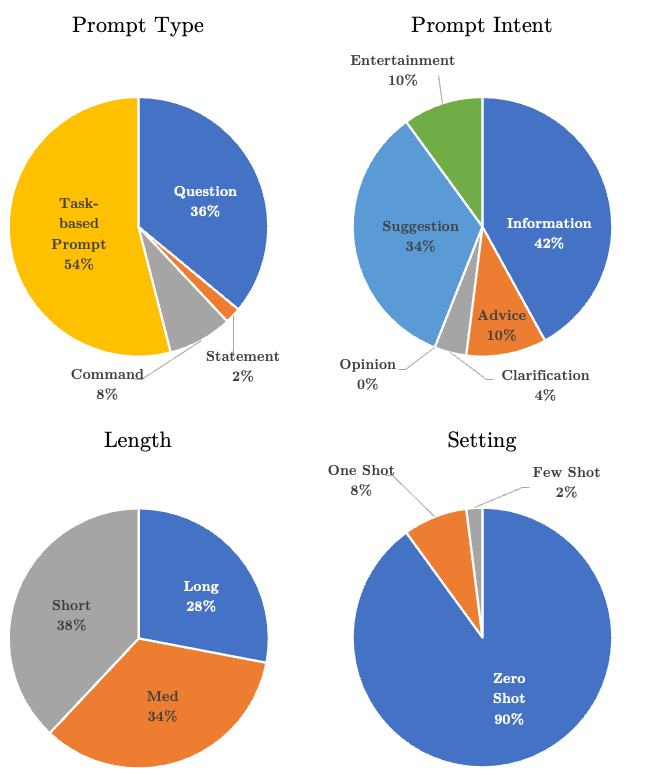
\includegraphics[width=0.475\textwidth]{images/charts1}
    \caption{ShareGPT Prompt Analysis Categories 1--4}
    \label{fig:chatgpt-categories-1}
\end{figure}
\vspace*{\fill}
\begin{figure}[]
    \centering
    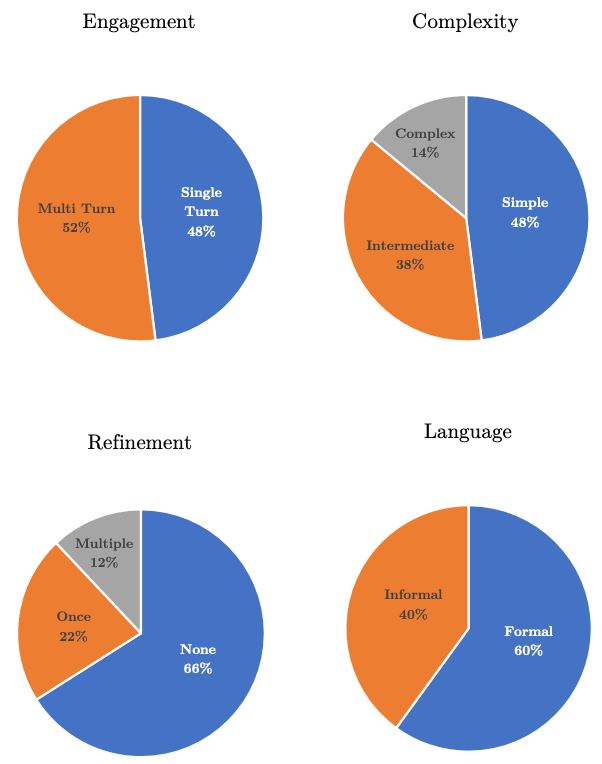
\includegraphics[width=0.475\textwidth]{images/charts2}
    \caption{ShareGPT Prompt Analysis Categories 5--8}
    \label{fig:chatgpt-categories-2}
\end{figure}
\begin{figure}[t]
    \centering
    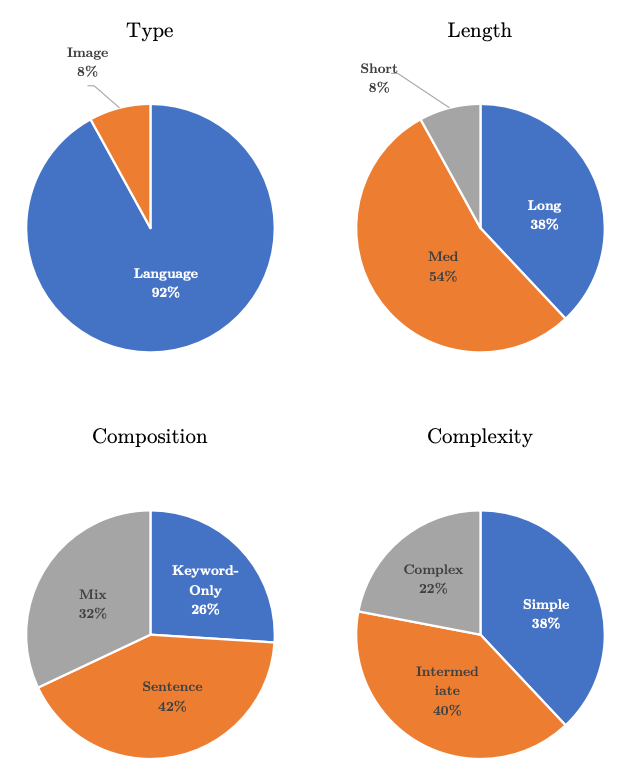
\includegraphics[width=0.475\textwidth]{images/charts3}
    \caption{Midjourney Prompt Analysis Categories 1--4}
    \label{fig:midjourney-categories-1}
\end{figure}
\begin{figure}[h]
    \centering
    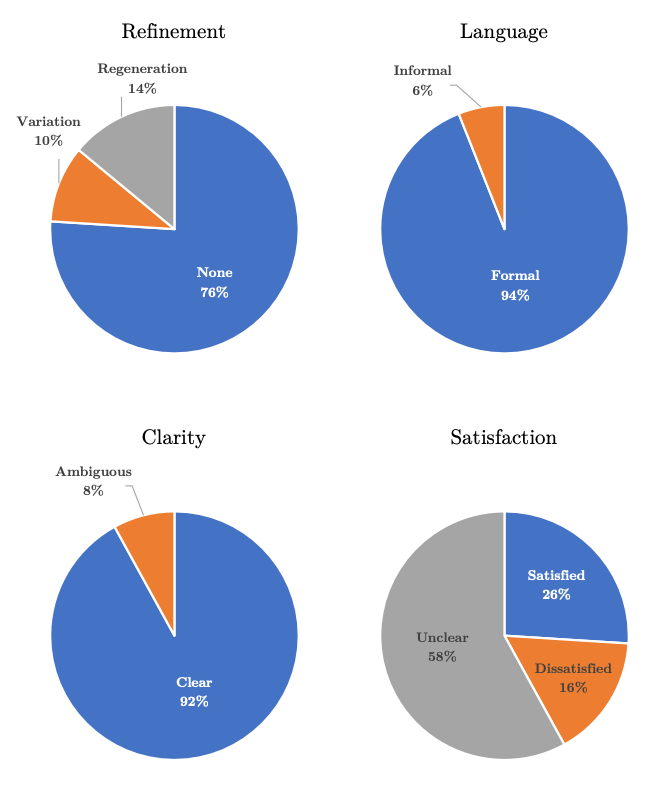
\includegraphics[width=0.475\textwidth]{images/charts4}
    \caption{Midjourney Prompt Analysis Categories 5--8}
    \label{fig:midjourney-categories-2}
\end{figure}

% TODO make an own subsection on difficulties of ordinary users in understanding how LLMs interpret
% natural language? in this subsec, we could focus on the example also displayed on midjourneys
% website: " If you ask for a party with “no cake,” your image will probably include a cake"
